\section{Whole-Part}


Das Whole-Part Design Pattern hilft beim Zusammensetzen von Komponenten welche zusammen eine semantische Einheit bilden. Die zusammengesetzte Einheit, das Whole (das Ganze), kapselt seine Bestandteile, die Parts (die Teile), organisiert ihre Zusammenarbeit und stellt eine gemeinsame Schnittstelle (Interface) zur Verfügung. Direkter Zugriff auf die Parts ist nicht möglich.

\subsection*{Exmaple}


Ein CAD-System für 2D- und 3D-Modellierung erlaubt Ingenieruen grafische Objekte interaktiv zu entwerfen. In solchen Systemen sind die meisten grafischen Objekte aus anderen Objekten zusammengesetzt. Ein Aut zum Beispiel besteht aus mehreren kleineren Objekten, wie Räder oder Fenster, welche wiederum aus mehreren noch kleineren Objekten bestehen können, wie Kreise oder Polygone. Das Auto-Objekt ist verantwortlich für die Funktionalität des Autos als ganzes, wie das Rotieren oder Zeichnen.

\subsection*{Context}


Zusammengesetzte Objekte implementieren.

\subsection*{Problem}


In fast jedem Software Sytem existieren Objekte welche aus anderen Objekten zusammengesetzt sind. Stellt man sich zum Beispiel in einer System zur chemischen Simulation ein Molekül-Objekt vor, so kann dieses als Graph von einzelnen Atom-Objekten implementiert sein. Solche zusammengesetzen Objekte (aggregate objects) repräsentieren nicht Mengen von lose gekoppelten Komponenten, sondern Einheiten welche mehr als nur die Summe ihrer Bestandteile sind. In diesem Beispiel hätte ein Molekül-Objekt Attribute, wie die chemischen Eigenschaften, und Methoden wie zur Rotation. Diese Attribute und Methode beziehen sich dabei auf das Molekül als semantische Einheit und nicht auf die einzelnen Atome aus welchem das Molekül besteht. Die Kombination der Einzelteile führt dazu das sich neue Eigenschaften herausbilden. Dieses Verhalten nennt sich "emergent behavior" (Emergentes Verhalten).

\subsection*{Forces}


\begin{itemize}
	\item Ein komplexes Objekt sollte zerlegbar in kleinere Objekte sein oder aus existierenden Objekten bestehen, um Wiederverwendbarkeit, Anpassbarkeit und die Rekombination der Bestandteile zu anderen Arten von zusammengesetzen Objekten erlauben.
	\item Clients sollten das zusammengesetze Objekt als eine Einheit sehen, welche keinen direkten Zugriff auf seine Bestandteile erlaubt.
\end{itemize}

\subsection*{Solution}


Führe eine Komponente ein welche kleinere Objekte kapselt und den direkt Zugriff von Clients auf diese unterbindet. Definiere eine Schnittstelle (Interface) welche das zusammengesetze Objekt als eine semantische Einheit repräsentiert.

Das allgemeine Prinzip des Whole-Part Patern ist anwendbar auf die Organisation von drei Arten von Beziehungen:

\begin{itemize}
	\item Assembly-Parts Beziehung, bei welchem ein Produkt in seine Bestandteile unterteilt wird. Alle Teile sind stark integriert. Die Anzahl und der Typ der Subassemblies ist vordefiniert und variert nicht.
	\item Container-Contents Beziehung, bei welcher das zusammengesetze Objekt durch einen Container repräsentiert wird. Zum Beispiel ein Post-Paket mit inhalt. Der Inhalt ist weniger stark gekopelt als die Bestandteile bei der Assembly-Parts Beziehung. Der Inhalt könnte auch dynamisch hinzugefügt oder entfert werden .
	\item Collection-Members Beziehung, welche Hilft ähnliche Objekte zu gruppieren, wie zum Beispiel die Mitglieder einer Organisation. Die Collection stellt Funktionalität zur Verfügung um über die Mitglieder zur iterieren und Operationen an ihnen auszuführen. Es gibt keine Unterscheidung zwischenen den einzelnen Mitgliedern der Collection, alle werden gleich behandelt.
\end{itemize}

Diese Beziehungen entsprechen den Beziehungen in der realen Welt. Wenn wir Software modellieren ist es nicht immer offensichtlich welche Beziehung verwendet werden sollte. Welche Beziehung die beste ist hängt mit der gewünschten Benutzung zusammen.
Es ist wichtig zu wissen das diese Kategorien Beziehungen zwischen Objekten und nicht Datentypen definieren.

\subsection*{Structure}


\begin{figure}[H]
	\centering
	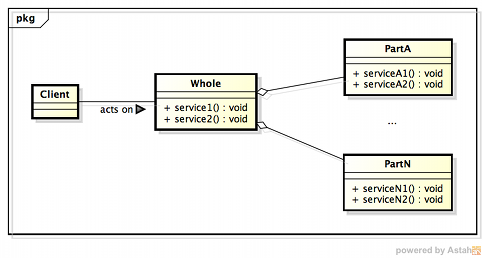
\includegraphics[width=0.7\textwidth]{content/posa1/images/whole-part-classes.png}
	\caption{Whole Part}
\end{figure}


Das Whole-Part Pattern besteht aus zwei Teilnehmern: das \textit{Whole}-Objekt repräsentiert eine Zusammensetzung von kleineren Objekten, welche \textit{Parts} genannt werden.

Einige Methoden des Whole-Objekts können auch nur Platzhalter für Dienste von bestimmten Parts sein. Wenn eine solche Methode aufgerufen wird, ruft das Whole den entsprechenden Dienst (Service) des Parts auf und gibt das Ergebnis an den Client zurück.

\subsection*{Dynamics}


Ein grafisches, zusammengesetztes Objekt soll rotiert werden.

\begin{itemize}
	\item Der Client ruft die Rotate-Methode des Whole-Objekts auf.
	\item Das Whole-Objekt ruft die Rotate-Methode jedes seiner Part-Objekte auf.
\end{itemize}

\subsection*{Implementation}


\begin{enumerate}
	\item Entwirf die öffentliche Schnittstelle des Whole-Objekts.
	\item Unterteile das Whole-Objekt in Part-Objekte oder erzeuge es aus existierenden Objekten. Dazu lässt sich ein Bottom-Up- oder ein Top-Down-Ansatz anwenden.
	\item Beim Bottom-Up-Ansatz, benutze existirende Parts von Komponenten-Bibliotheken oder Class-Libraries und spezifiere ihre Zusammenarbeit. Falls nicht die ganze Funktionalität durch solche Parts abgedeckt werden kann, kann es nötig sein den Top-Down-Ansatz anzuwenden, um die fehlenden Parts zu implementieren.
	\item Beim Top-Down-Ansatz, unterteile die Dienste des Whole-Objekts in kleinere, zusammenarbeitende Dienste und weise sie einzelnen Parts zu.
	\item Spezifiere die Dienste des Whole-Objekts durch Dienste der Parts. Es gibt zwei Möglichkeiten einen Dienst eines Parts aufzurufen: 1) Der Request des Clients muss nichts über den Kontext des Wholes wissen. Dies führt zu einer losen Koplung zwischen Whole und Part. 2) Die Delegation an das Part muss Kontext-Informationen mitgeben.
	\item Implementiere die Parts.
	\item Implementiere das Whole.
\end{enumerate}


\subsection*{Variants}

\begin{itemize}
	\item Shared Parts: Bei dieser Variante kann ein Part von mehreren Whole-Objekten geteilt werden.
	\item Assembly-Parts: Das Whole repräsentiert eine Gruppe von kleineren Objekten.
	\item Container-Contents: Dabei ist ein Container verantwortlich die verschiedenen Inhalte zu verwalten. Im Gegensatz zum Assembly-Part können Inhalte dynamisch hinzugefügt oder entfernt werden.
	\item Collection-Members: Bei dieser spezialisierung der Vontainer-Contents-Variante sind alle Part-Objekte vom selben Typ.
	\item Composite Pattern: Sowohl Whole, als auch Part implementieren die selbe Schnittstelle (interface) und können so beliebig verschachtelt werden.
\end{itemize}

\begin{figure}[H]
	\centering
	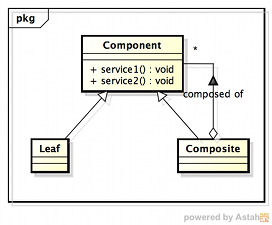
\includegraphics[width=0.7\textwidth]{content/posa1/images/whole-part-composite.png}
	\caption{Whole Part Composite}
\end{figure}

\subsection*{Known Uses}


\begin{itemize}
	\item Object-Oriented Applications, graphical Editors
	\item Object-Oriented Collection Libraries
	\item Graphical user interface toolkits (Fresco, ET++)
\end{itemize}

\subsection*{Consequences}


\subsubsection*{Benefits}


\begin{itemize}
	\item Änderbarkeit der Parts
	\item Separation of concerns
	\item Wiederverwendbarkeit
\end{itemize}

\subsubsection*{Liabilities}

\begin{itemize}
	\item Effizienzverlust durch Indirektion
	\item Komplexe Unterteilung in Parts
\end{itemize}

\subsection*{See also}

\begin{itemize}
	\item Composite Design Pattern (GOF)
	\item Facade Design Pattern (GOF)
\end{itemize}

